\section{Stable Diffusion}
Latent Diffusion adı verilen özel bir modele dayanmaktadır. Model başlangıçta LAION-5B veriseti ile 512x512 boyutunda görüntüler ile eğitilmiştir. Metin tabanlı istemlerden yüksek kaliteli görüntüler üreten bir modeldir. Text Encoder, U-Net ve VAE'den oluşur. 
\begin{enumerate}
    \item CLIP modeli ile prompt kodlanır.
    \item Rastgele bir gürültü oluşturulur.
    \item U-Net ile gürültü ve kodlanmış metni girdi olarak kullanılır. Burdaki çıktı görüntünün gizli temsilidir.
    \item VAE ile görüntünün gizli temsili çözülerek görüntü orijinal boyuta döndürülür.
\end{enumerate}

\begin{figure}[ht]
    \centering
    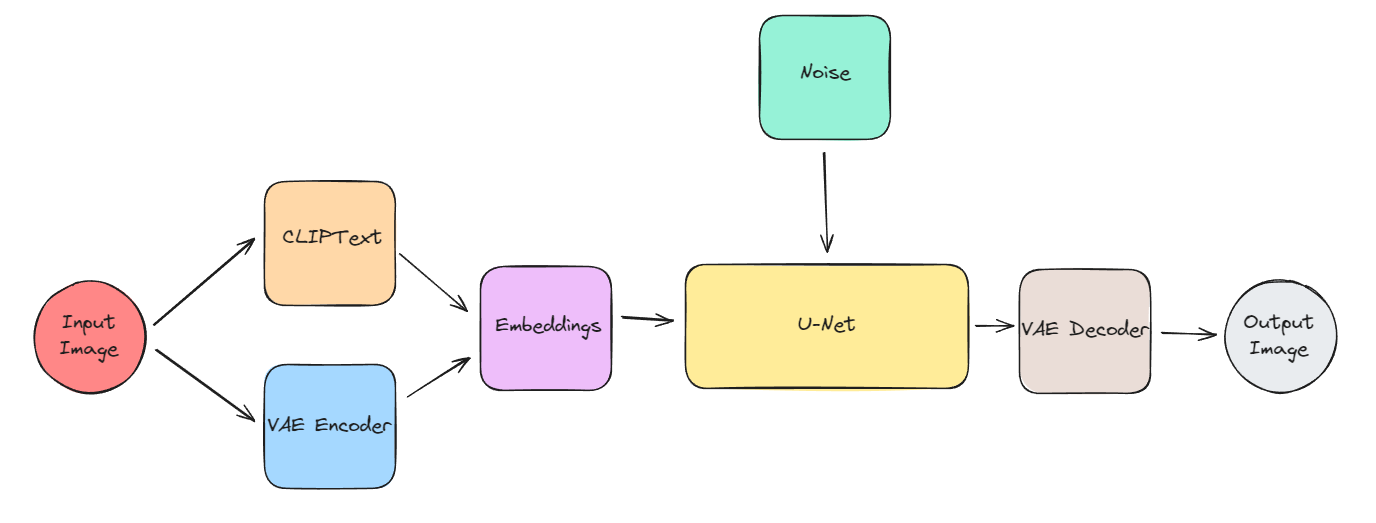
\includegraphics[width=0.9\textwidth]{images/stable_diffusion_architecture.png}
    \caption{Stable Diffusion mimarisi.}
    \label{fig:enter-label}
\end{figure}

\subsection{CLIP}
OpenAI tarafından geliştirilmiştir. CLIP (Contrastive Language-Image Pre-training) hem görüntüler hem de metinler için bir gömülü uzayda eğitilmiş, görsel ve metin veriler arasındaki ilişkileri keşfetmek için kullanılır. Metinlerin belirli bir uzayda gömülmesini sağlra ve görsel verilerle karşılaştırılabilir bir şekilde temsil edilmesini sağlar. Stable Diffusion'da CLIP tarafından üretilen vektörler modelin Attention katmanlarından bir çok kez geçer. Bu attention layer'lar cross-attention prensibiyle çalışır. 

\subsection{Cross-Attention}
Cross-Attention, bir veri kümesindeki her bir elemanın, başka bir veri kümesindeki tüm elemanlara olan dikkatini ölçer. Bu, bir veri kümesindeki her bir elemanın, diğer veri kümesindeki en uygun karşılıkları veya ilişkili elemanları belirlemesine yardımcı olur. Stable Diffusion'da bir resmin belirli bir metin açıklaması ile ilişkilendirilmek için kullanılır.

\subsection{U-Net}
Görüntü oluşturma aşamasında kullanılır. Gürültüden yola çıkarak gerçekçi bir görüntü oluşturur. 

\subsection{VAE}
Encoder, 512x512 boyutundaki görüntü 64x64 boyutuna düşürülerek U-Net modeline girdi olarak gönderilir. Decoder, gizli temsili tekrar görüntüye dönüştürür. Reverse Diffusion sonrası üretilen gürültüden arındırılmış temsilleri görüntüye dönüştürür.

\newpage